% Graphical overview (Fig. 1) -- compile with pdflatex, then
%   pdftops -eps Fig1_overview.pdf Fig1.eps
% Designed for a printed width of about 12-13 cm (scale close to 1).
\documentclass[border=3pt]{standalone}
\usepackage{amsmath,amssymb}
\usepackage{tikz}
\usetikzlibrary{arrows.meta,calc}
\usepackage[scaled=0.92]{helvet}
\renewcommand{\familydefault}{\sfdefault}
\usepackage{sansmath}\sansmath

\definecolor{water}{RGB}{214,232,250}
\definecolor{heat}{RGB}{253,226,200}
\definecolor{oil}{RGB}{222,206,170}
\definecolor{grain}{RGB}{165,165,165}
\definecolor{sorb}{RGB}{200,30,30}
\definecolor{cfront}{RGB}{200,30,30}
\definecolor{tfront}{RGB}{0,120,0}
\definecolor{sline}{RGB}{0,60,200}
\definecolor{boxA}{RGB}{235,242,252}
\definecolor{boxB}{RGB}{252,240,228}
\definecolor{boxC}{RGB}{236,247,236}

\begin{document}
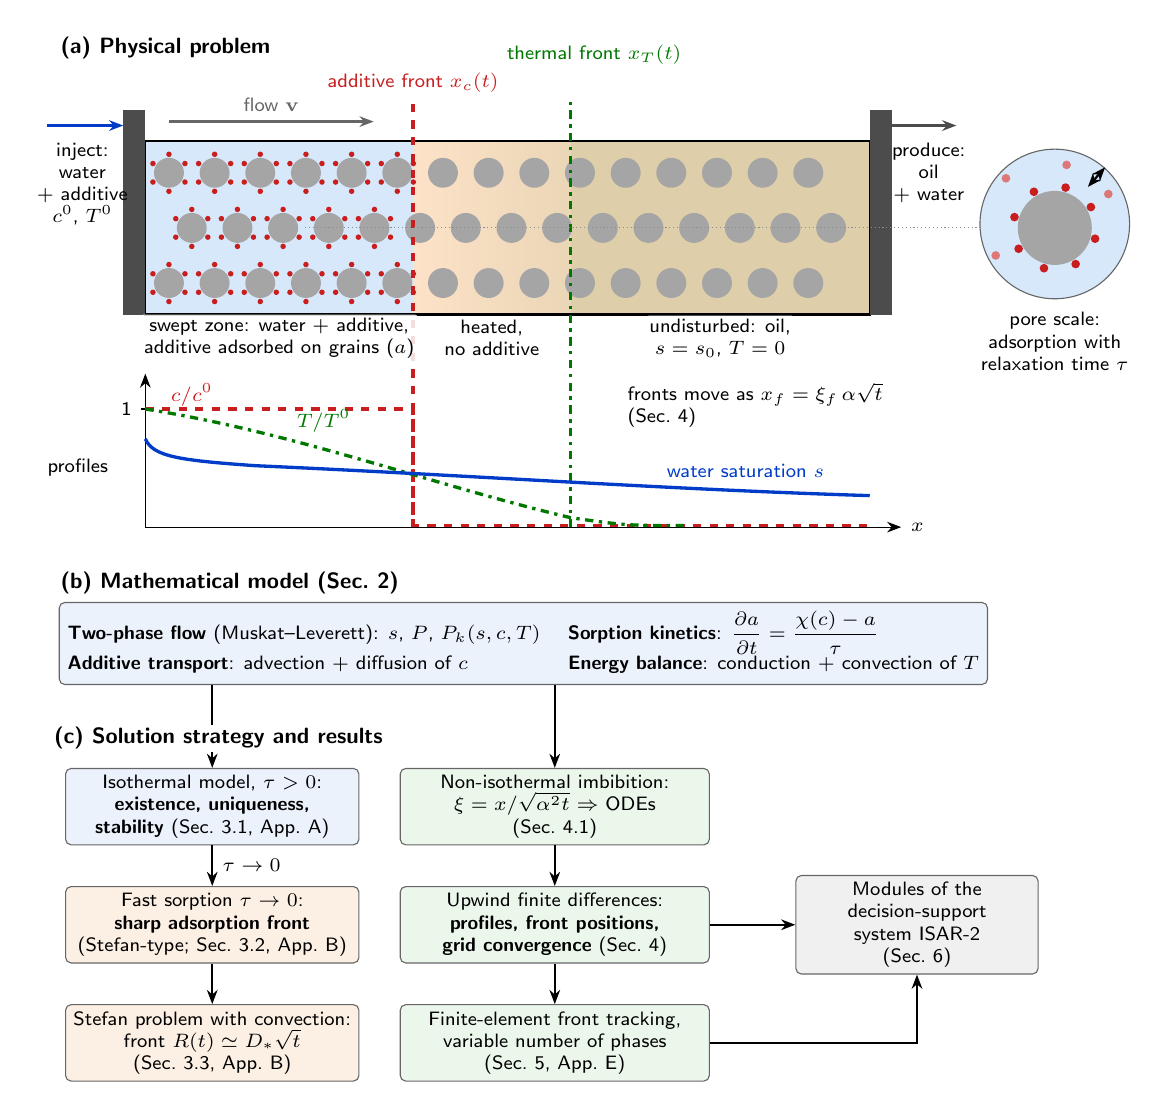
\begin{tikzpicture}[
  >={Stealth[length=1.8mm]},
  lab/.style={font=\scriptsize, align=center},
  small/.style={font=\scriptsize, align=center},
  panel/.style={font=\footnotesize\bfseries, anchor=north west},
  sbox/.style={draw=black!60, rounded corners=2pt, font=\scriptsize,
               align=flush center, inner sep=2.5pt, text width=#1},
]

% ======================================================================
% (a) Physical problem
% ======================================================================
\node[panel] at (-0.3,6.35) {(a) Physical problem};

\def\xL{0.9}\def\xR{10.1}\def\xc{4.3}\def\xT{6.3}
\fill[water] (\xL,2.7) rectangle (\xc,4.9);
\shade[left color=heat, right color=heat!40!oil] (\xc,2.7) rectangle (\xT,4.9);
\fill[oil] (\xT,2.7) rectangle (\xR,4.9);
\draw[thick] (\xL,2.7) rectangle (\xR,4.9);

% grains
\foreach \i in {0,...,15}{
  \foreach \j in {0,1,2}{
    \pgfmathsetmacro{\xx}{1.2+0.58*\i+0.29*mod(\j,2)}
    \pgfmathsetmacro{\yy}{3.1+0.7*\j}
    \pgfmathparse{\xx<9.9 ? 1 : 0}
    \ifnum\pgfmathresult=1
      \fill[grain] (\xx,\yy) circle (0.19);
      \pgfmathparse{\xx<4.15 ? 1 : 0}
      \ifnum\pgfmathresult=1
        \foreach \ang in {30,90,150,210,270,330}{
          \fill[sorb] ($(\xx,\yy)+(\ang:0.235)$) circle (0.035);
        }
      \fi
    \fi
  }
}

% wells
\fill[black!70] (0.62,2.7) rectangle (\xL,5.3);
\fill[black!70] (\xR,2.7) rectangle (10.38,5.3);
\draw[->, very thick, sline] (-0.35,5.1) -- (0.62,5.1);
\node[small, anchor=north] at (0.1,5.0) {inject:\\ water\\ $+$ additive\\ $c^0$, $T^0$};
\draw[->, very thick, black!70] (10.38,5.1) -- (11.2,5.1);
\node[small, anchor=north] at (10.85,5.0) {produce:\\ oil\\ $+$ water};

% flow arrow
\draw[->, thick, black!60] (1.2,5.15) -- (3.8,5.15) node[midway, above, small] {flow $\mathbf v$};

% fronts
\draw[cfront, very thick, dashed] (\xc,0) -- (\xc,5.4);
\draw[tfront, very thick, dash dot] (\xT,0) -- (\xT,5.4);
\node[small, text=cfront, anchor=south] at (\xc,5.4) {additive front $x_c(t)$};
\node[small, text=tfront, anchor=south] at (\xT+0.3,5.75) {thermal front $x_T(t)$};

% zone labels
\tikzset{zl/.style={lab, fill=white, fill opacity=0.85, text opacity=1, rounded corners=1pt, inner sep=1.2pt}}
\node[zl] at (2.6,2.4) {swept zone: water $+$ additive,\\ additive adsorbed on grains ($a$)};
\node[zl] at (5.3,2.4) {heated,\\ no additive};
\node[zl] at (8.2,2.4) {undisturbed: oil,\\ $s=s_0$, $T=0$};

% pore-scale inset
\begin{scope}[shift={(12.45,3.85)}]
  \draw[black!60, fill=water] (0,0) circle (0.95);
  \fill[grain] (0,-0.05) circle (0.47);
  \foreach \ang in {30,75,120,165,210,255,300,345}{
    \fill[sorb] ($(0,-0.05)+(\ang:0.53)$) circle (0.055);
  }
  \foreach \p in {(-0.62,0.58),(0.15,0.75),(0.68,0.38),(-0.75,-0.4)}{
    \fill[sorb!60] \p circle (0.055);
  }
  \draw[<->, thick] (0.42,0.47) -- (0.64,0.72);
  \node[small, anchor=north] at (0,-1.0) {pore scale:\\ adsorption with\\ relaxation time $\tau$};
\end{scope}
\draw[black!45, densely dotted] (2.93,3.8) -- (11.5,3.8);

% sketched profiles aligned with the reservoir
\draw[->] (\xL,0) -- (10.5,0) node[right, small] {$x$};
\draw[->] (\xL,0) -- (\xL,1.95);
\draw (0.85,1.5) -- (0.95,1.5) node[pos=0, left, small] {1};
\node[small, anchor=east] at (0.55,0.75) {profiles};
\draw[cfront, very thick, dashed] (\xL,1.5) -- (\xc,1.5) -- (\xc,0.02) -- (10.1,0.02);
\draw[tfront, very thick, dash dot] (\xL,1.5) .. controls (2.8,1.2) and (4.5,0.55) .. (\xT,0.12)
    .. controls (7.0,0.02) .. (7.8,0.02);
\draw[sline, very thick] (\xL,1.12) .. controls (1.0,0.9) and (1.3,0.85) .. (2.3,0.78)
    .. controls (5,0.66) and (7.5,0.48) .. (10.1,0.4);
\node[small, text=cfront, anchor=west] at (1.1,1.68) {$c/c^0$};
\node[small, text=tfront, anchor=west] at (2.7,1.35) {$T/T^0$};
\node[small, text=sline,  anchor=west] at (7.4,0.72) {water saturation $s$};
\node[small, anchor=west, align=left] at (6.9,1.55) {fronts move as $x_f=\xi_f\,\alpha\sqrt{t}$\\ (Sec.~4)};

% ======================================================================
% (b) Mathematical model
% ======================================================================
\node[panel] at (-0.3,-0.45) {(b) Mathematical model (Sec.~2)};
\node[draw=black!60, rounded corners=2pt, fill=boxA, anchor=north west, font=\scriptsize,
      inner sep=3pt] (mod) at (-0.2,-0.95) {%
  \begin{tabular}{@{}l@{\hspace{10pt}}l@{}}
  \textbf{Two-phase flow} (Muskat--Leverett): $s$, $P$, $P_k(s,c,T)$ &
  \textbf{Sorption kinetics}: $\dfrac{\partial a}{\partial t}=\dfrac{\chi(c)-a}{\tau}$\\[2pt]
  \textbf{Additive transport}: advection $+$ diffusion of $c$ &
  \textbf{Energy balance}: conduction $+$ convection of $T$
  \end{tabular}};

% ======================================================================
% (c) Solution strategy
% ======================================================================

\def\ya{-3.55}\def\yb{-5.05}\def\yc{-6.55}
\node[sbox=3.55cm, fill=boxA] (iso)  at (1.75,\ya)
  {Isothermal model, $\tau>0$:\\ \textbf{existence, uniqueness,}\\ \textbf{stability} (Sec.~3.1, App.~A)};
\node[sbox=3.55cm, fill=boxB] (stef) at (1.75,\yb)
  {Fast sorption $\tau\to0$:\\ \textbf{sharp adsorption front}\\ (Stefan-type; Sec.~3.2, App.~B)};
\node[sbox=3.55cm, fill=boxB] (conv) at (1.75,\yc)
  {Stefan problem with convection:\\ front $R(t)\simeq D_*\sqrt{t}$\\ (Sec.~3.3, App.~B)};

\node[sbox=3.75cm, fill=boxC] (ss) at (6.1,\ya)
  {Non-isothermal imbibition:\\ $\xi=x/\sqrt{\alpha^2 t}$ $\Rightarrow$ ODEs\\ (Sec.~4.1)};
\node[sbox=3.75cm, fill=boxC] (fd) at (6.1,\yb)
  {Upwind finite differences:\\ \textbf{profiles, front positions,}\\ \textbf{grid convergence} (Sec.~4)};
\node[sbox=3.75cm, fill=boxC] (fe) at (6.1,\yc)
  {Finite-element front tracking,\\ variable number of phases\\ (Sec.~5, App.~E)};

\node[sbox=2.9cm, fill=black!6] (dss) at (10.7,\yb)
  {Modules of the\\ decision-support\\ system ISAR-2\\ (Sec.~6)};

\draw[->, thick] (iso) -- node[right, small] {$\tau\to0$} (stef);
\draw[->, thick] (stef) -- (conv);
\draw[->, thick] (ss) -- (fd);
\draw[->, thick] (fd) -- (fe);
\draw[->, thick] (fd.east) -- (dss.west);
\draw[->, thick] (fe.east) -| (dss.south);
\draw[->, thick] (mod.south -| iso) -- (iso.north);
\draw[->, thick] (mod.south -| ss) -- (ss.north);
\node[panel, fill=white, inner sep=1pt] at (-0.3,-2.5) {(c) Solution strategy and results};

\end{tikzpicture}
\end{document}
